\documentclass{report}[12pt]
\usepackage{amssymb}
\usepackage{amsmath}
\usepackage{geometry}
\usepackage{cite}
\usepackage[utf8]{inputenc}
\usepackage{graphicx}
\graphicspath{ {images/} }
\usepackage{float}
\usepackage{fullpage}

\usepackage{siunitx}
\usepackage{enumitem}
\usepackage{textcomp}
\usepackage{setspace}
\usepackage{subcaption}


\usepackage{color}   
\usepackage{hyperref}
\hypersetup{
    colorlinks=true, 
    linktoc=all,     
    linkcolor=blue,  
}

\author{Anurag Gupta (183230006) \\ Ponala Venkata Eswara Srisai
(183230008)\\ Sudhakar Kumar (183236001)\\ Kishan Chouhan (183230015)}
\title{Systems and Control Engineering Laboratory (SC 626) \\ Kilobotics}

\begin{document}
\maketitle
\tableofcontents
\thispagestyle{empty}
\mbox{}
\newpage

\chapter{Overview of Kilobots}

Kilobots are low cost robots designed at \textbf{Harvard University's Self-Organizing Systems Research Lab} \url{http://www.eecs.harvard.edu/ssr}. The robots are designed to make testing collective algorithms on hundreds or thousands of robots accessible to robotics researchers.\\

Though the Kilobots are low-cost, they maintain abilities similar to other collective robots. These abilities include differential drive locomotion, on-board computation power, neighbor-to-neighbor communication, neighbor-to neighbor distance sensing, and ambient light sensing. Additionally they are designed to operate such that no robot requires any individual attention by a human operator. This makes controlling a group of Kilobots easy, whether there are 10 or 1000 in the group.
 
\section{Specifications of Kilobot}
Kilobots (Figure \ref{fig:kilobot}) are low cost, low power, tiny robots designed by Harvard University's Self Organizing Systems Research Lab with the aim of making testing collective algorithms accesible to researchers \cite{kilobotics_manual}. It has following specifications:
\begin{itemize}
\item \textbf{Processor}: ATmega 328p (8bit @ 8MHz)
\item \textbf{Memory}: 
\begin{itemize}
\item 32 KB Flash -- used for both user program and bootloader 
\item 1KB EEPROM -- for storing calibration values and other non-volatile data and 2KB SRAM
\end{itemize}
\item \textbf{Battery}: Rechargeable Li-Ion 3.7V, for a 3 months autonomy in
sleep mode. Each Kilobot has a built-in charger circuit which charges the onboard battery when +6 volts is applied to any of the legs, and GND is applied to the charging tab. 
\item \textbf{Charging}: Kilobot charger for 10 robots simultaneously
\item \textbf{Communication}: Kilobots can communicate with neighbors up to 7 cm away by reflecting infrared (IR) light off the ground surface (Figure \ref{fig:comm}). 
\item \textbf{Sensing}: one IR sensor and one light sensor 
\begin{itemize}
\item When receiving a message, distance to the transmitting Kilobot can be determined using received signal strength. The distance depends on the surface used as the light intensity is used to compute the value.
\item The brightness of the ambient light shining on a Kilobot can be detected.
\item A Kilobot can sense its own battery voltage.
\end{itemize}
\item \textbf{Movement}: Each Kilobot has 2 vibration motors, which are
independently controllable, allowing for differential drive
of the robot. Each motor can be set to 255 different power
levels. The movement happens via \emph{stick and slip} mechanism
\item \textbf{Light}: Each Kilobot has a red/green/blue (RGB) LED pointed
upward, and each color has 3 levels of brightness control. 
\item \textbf{Software}: The Kilobot Controller software (kiloGUI) is available for controlling the controller board, sending program files to
the robots and controlling them.
\item \textbf{Programming}: C language with WinAVR compiler combined with Eclipse or the online Kilobotics editor (\url{https://www.kilobotics.com/editor})
\item \textbf{Dimensions}: diameter: 33 mm, height 34 mm (including the legs,
without recharge antenna). 
\end{itemize}

\begin{figure}[H]
	\begin{subfigure}{0.45\textwidth}
		\centering
		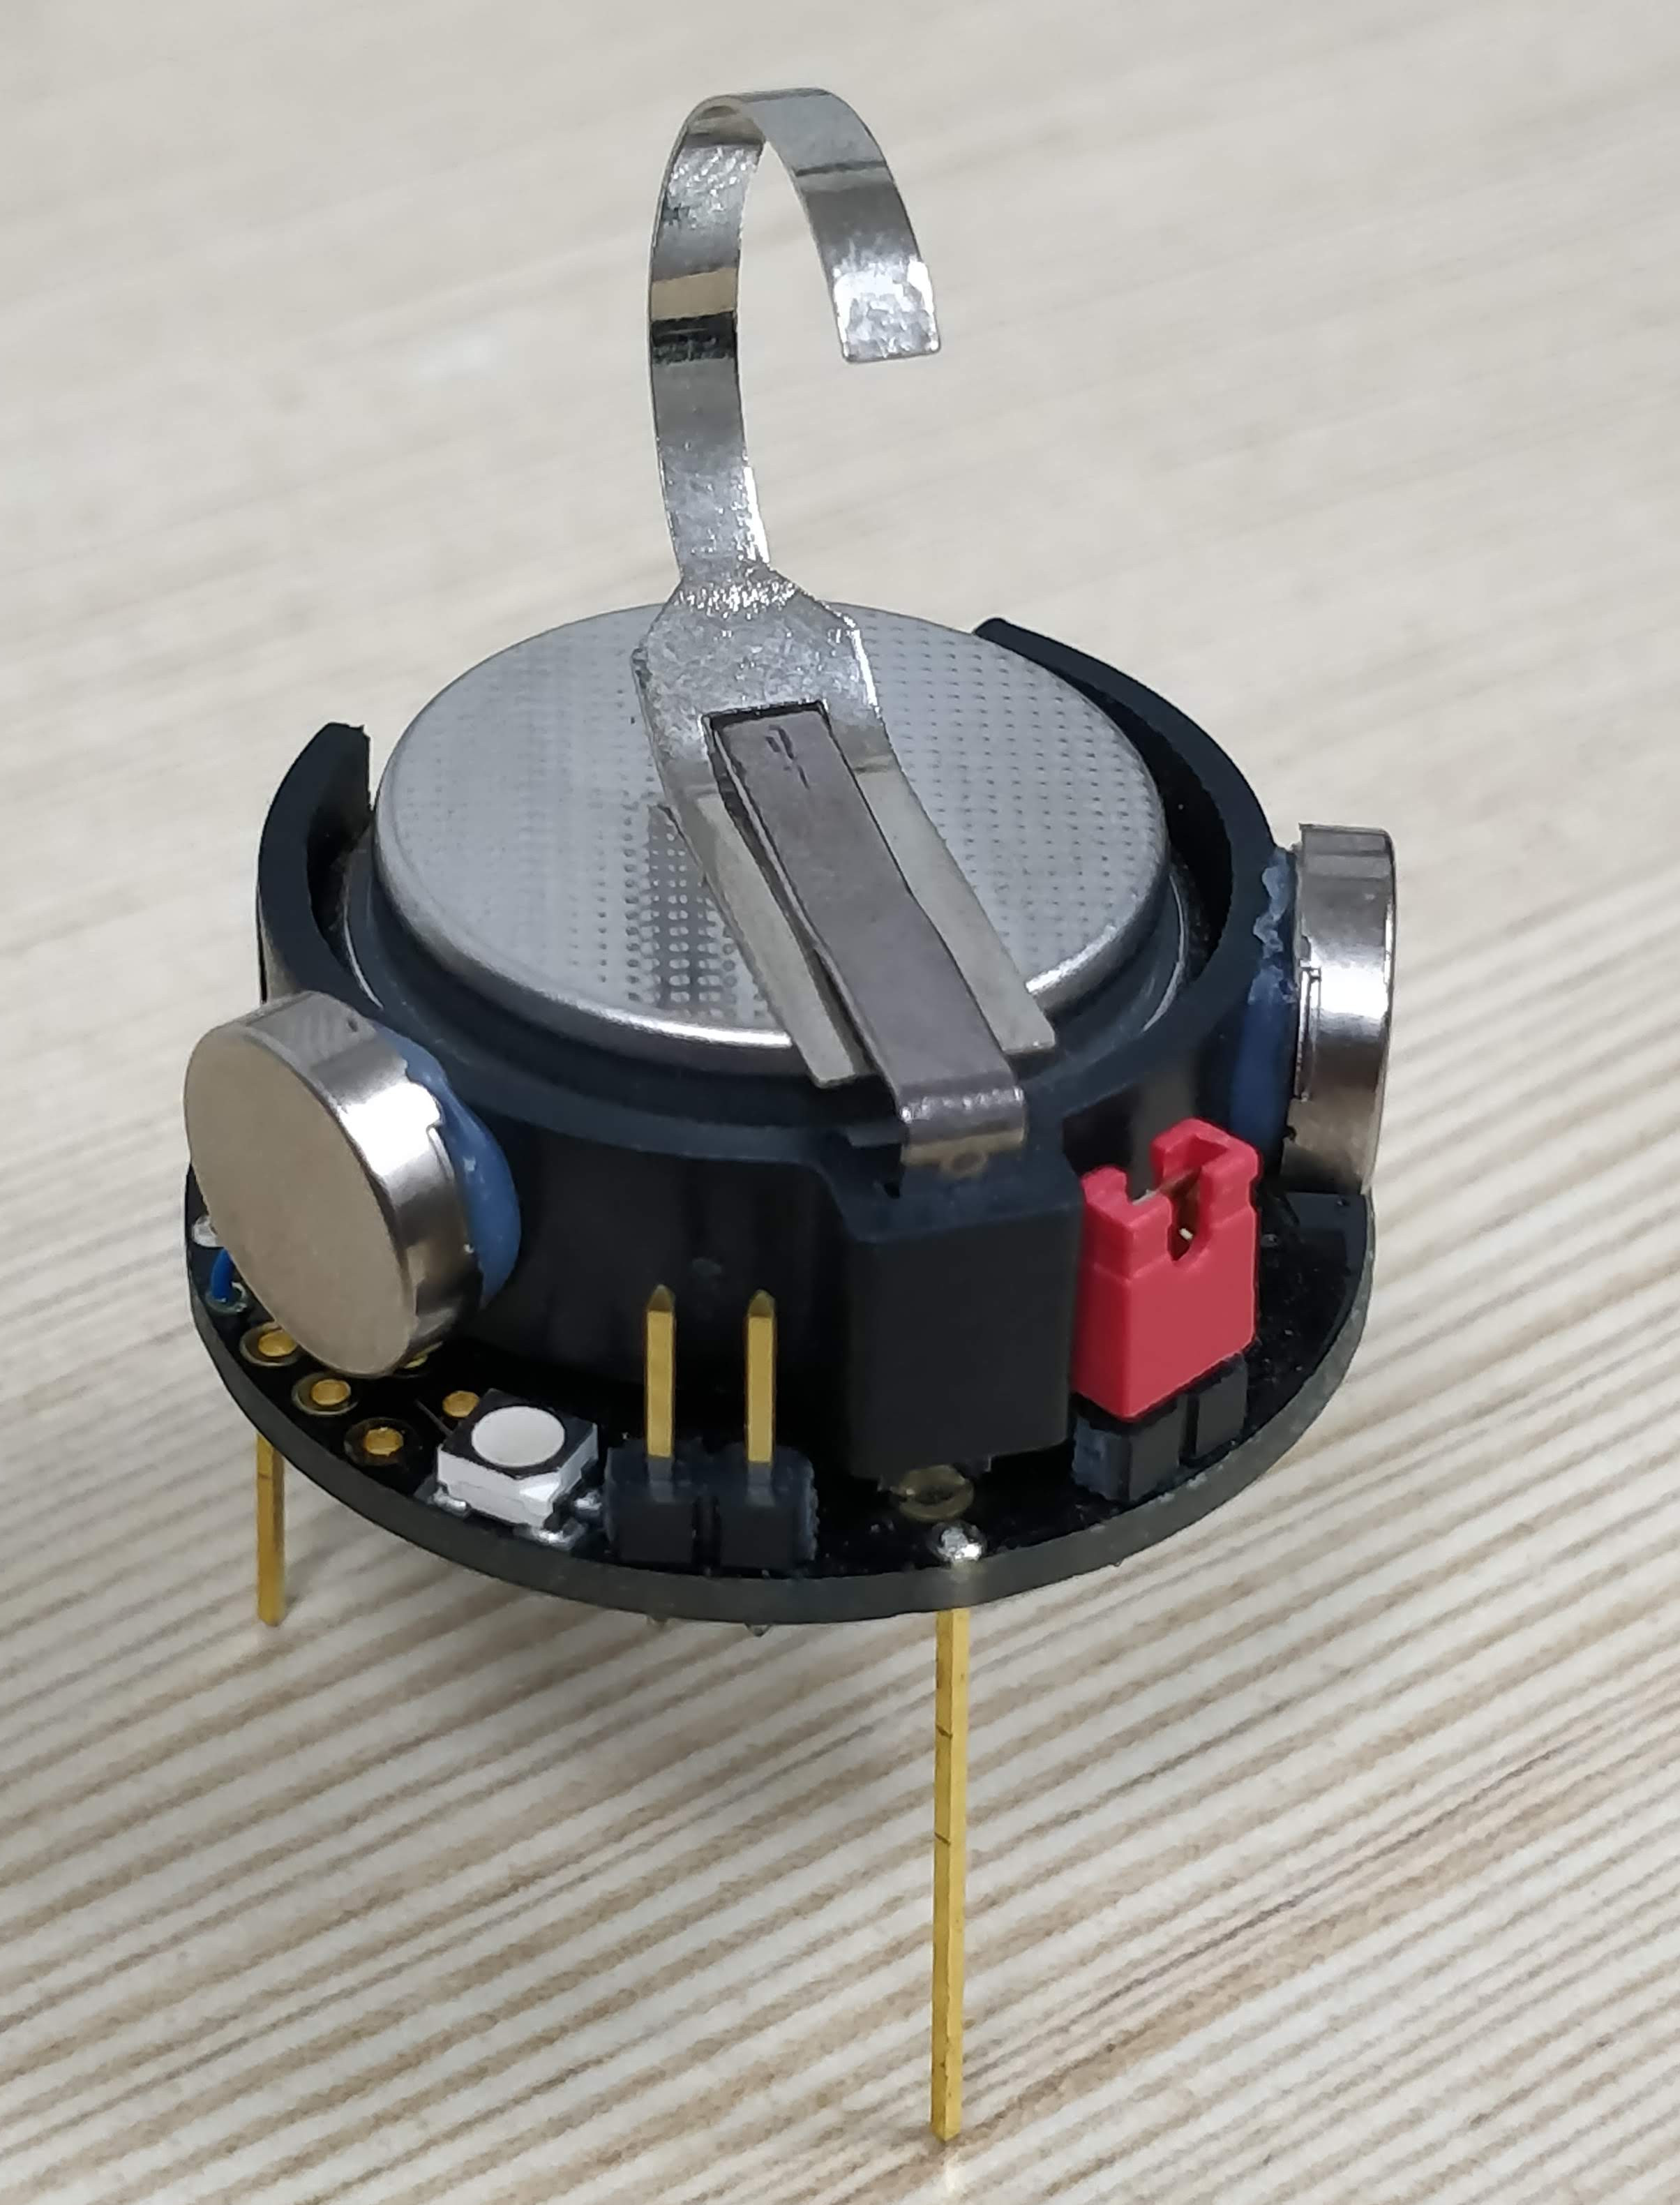
\includegraphics[scale=0.04]{images/kilobots}
		\caption{Kilobot}
		\label{fig:kilobot}
	\end{subfigure}
	\begin{subfigure}{0.45\textwidth}
		\centering
		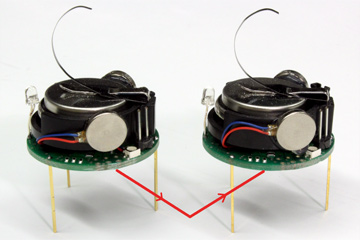
\includegraphics[scale=0.5]{images/comm}
		\caption{IR sensing (Source \cite{kilobotics_manual})}
        \label{fig:comm}
	\end{subfigure}
\end{figure}

\section{Hardware/ Software Requirement}
The required hardware and software to use the board and develop programs are described below.\\\\
Required hardware:
\begin{itemize}
\item Computer with an USB port
\item Kilobot robot
\item Over-head controller (OHC)
\item Kilobot charger
\end{itemize}

\noindent Required software:
To start programming the Kilobot with the new version from kilobotics, we  have two solutions.
\begin{itemize}
\item Online editor \url{https://www.kilobotics.com/editor}.
\item Install WinAVR and Eclipse to compile the whole library on your computer \url{https://github.com/mgauci/kilobot_notes/blob/master/eclipse_winavr_setup/eclipse_winavr_setu
p.md}. 
\end{itemize}
We have used online editor for our labs. 

\section{Over-head Controller}
To make a robot scalable to large collective sizes, all the operations of the robot must work on the collective as a whole \cite{mclurkin2006speaking}, and not require any individual attention to the robot, such as pushing a switch or plugging in a charging cable for each robot. In other words, all collective operations must be scalable. In the case of Kilobots, instead of plugging in a programming
cable to each robot in order to update its program, each can
receive a program via an infrared communication channel.
This allows an overhead infrared transmitter  (Figure \ref{fig:ohc}) to program all
the robots in the collective in a fixed amount of time, independent of the number of robots. 

\begin{figure}
    \centering
	\fbox{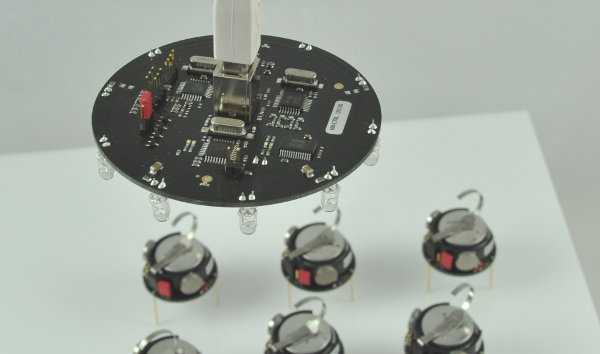
\includegraphics[scale=0.5]{images/ohc}}
	\caption{Overhead Controller (Source: \cite{kilobotics_manual})}
	\label{fig:ohc}
\end{figure}
\noindent Kilobots are unique in that they stay in ``sleep mode" until summoned by the overhead controller. A person can turn an entire swarm of Kilobots ``ON'' by sending out one signal -- as opposed to manually switching ``ON'' every robot.

\chapter{Kilobot Labs}

\section{Establishing communication between two Kilobots}
In this lab we will use the ability of two kilobots to communicate with each other. We will allocate one kilobot to be the speaker and the other kilobot to be the listener.
\subsection{Speaker}
 The objective of this part is to broadcast a fixed message, and blink magenta when we transmit. Here we introduce \texttt{message\_t} data structure, and the kilo\_message\_tx callback.
\begin{itemize}
\item A kilobot uses infrared (IR) to broadcast a message within an approximately circular radius of three body lengths.

\item  Multiple robots packed closely together will interfere the IR signals. So the kilobots use a variant of the CSMA/CD media access control method  to resolve the problems with interference.\par

Carrier-sense multiple access with collision detection (CSMA/CD) is a media access control method which uses carrier-sensing to delay transmissions until no other stations are transmitting. 
\end{itemize}

\noindent \textbf{Step 1}: Declare a variable called transmit\_msg of the structure type message\_t and add the function message\_tx() that returns the address of the message we declared (return $\And$transmit\_msg).
\newline
\newline
 \noindent \textbf{Step 2}: We will register this "callback" function in the kilobot main loop, and every time the kilobot is ready to send a message it will "interrupt" the main code and call the message\_tx() to get the message that needs to be sent.\par
 A callback is any executable code that is passed as an argument to other code, which is expected to call back the argument at a given time.
\begin{verbatim}
message_t transmit_msg;

message_t *message_tx() {
    return &transmit_msg;
} 

\end{verbatim}
\noindent \textbf{Step 3}:
 Use the setup() function to set the initial contents of the message and compute the message CRC value (used for error detection) through the function message\_crc(). The code below shows how to initialize a simple message. \par
 A cyclic redundancy check (CRC) is an error-detecting code which is used to detect accidental changes to raw data.
\begin{verbatim}
void setup() {
    transmit_msg.type = NORMAL;
    transmit_msg.data[0]=0;
    transmit_msg.crc = message_crc(&transmit_msg);
}
\end{verbatim}

\noindent \textbf{Step 4}:
 Now we will add some more code so that we can have the LED blink whenever the robot sends a message out. To do this we will declare a variable (often called a "boolean flag") called message\_sent. We will set this flag inside a function called message\_tx\_success() which is another callback function that only gets called when a message is finally successfully sent on a channel. Then we will clear this flag in the main loop where we will blink an LED to indicate that a message was sent. 
\begin{verbatim}
//At the top of the file, declare a "flag" for when a message is sent
int message_sent = 0;

// Add another function definition after your message_tx function
// (note that "void" means the function doesn't return any value)

void message_tx_success() {
   message_sent = 1;
}
\end{verbatim}

\noindent \textbf{Step 5}:
Then, in our program loop, write code to do this

\begin{verbatim}
// Blink led magenta when you get a message
if (message_sent == 1) {
    message_sent = 0;
    set_color(RGB(1,0,1));
    delay(100);
    set_color(RGB(0,0,0));
}
\end{verbatim}

\noindent \textbf{Step 6}:
Finally, we must register our message transmission functions with the kilobot library as follows:
\begin{verbatim}
int main() {
    kilo_init();
    kilo_message_tx = message_tx;
    kilo_message_tx_success = message_tx_success;
    kilo_start(setup, loop);

    return 0;
}

\end{verbatim}

\begin{figure}[H]
\begin{center}
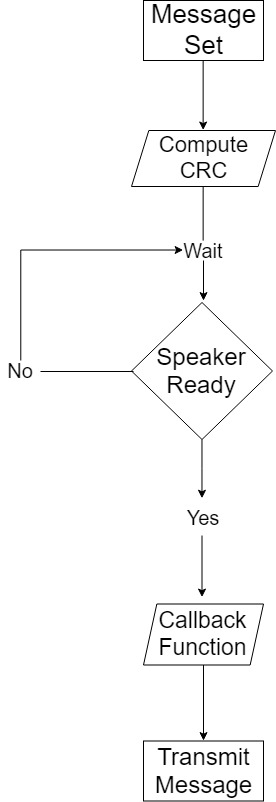
\includegraphics[scale=0.55]{speaker}
\caption{Broadcasting of a message}
\end{center}
\end{figure} 

\subsection{Listener}
The objective of this part is to blink yellow when a new message is received and introduce the kilo\_message\_rx callback and store incoming messages.
\newline
\newline
\noindent \textbf{Step 1}:
First declare a variable rcvd\_message of type message\_t to store any new incoming messages and a boolean variable called new\_message to indicate that a new message has been received.
\begin{verbatim}
int new_message = 0;
message_t rcvd_message;

void message_rx(message_t *msg, distance_measurement_t *dist) {
    rcvd_message = *msg;  //store the incoming message
    new_message = 1;      // set the flag to 1 to indicate that a new message arrived
}
\end{verbatim}

\noindent \textbf{Step 2}:
Check the flag in the program loop to see if a new message has arrived. If a new message has arrived, we will blink the LED yellow, and clear the flag.

\begin{verbatim}
void loop() {
    // Blink led yellow when you get a message
    if (new_message == 1) {
        new_message = 0;
        set_color(RGB(1,1,0));
        delay(100);
        set_color(RGB(0,0,0));
    }
}
\end{verbatim}
\noindent \textbf{Step 3}:
Modify our main section to register the message reception function with the kilobot library as follows:

\begin{verbatim}
int main() {
    kilo_init();
    kilo_message_rx = message_rx;
    kilo_start(setup, loop);

    return 0;
}
\end{verbatim}
\subsection{Demonstration}
Video of working demo of problem statement can be accessed using link in figure \ref{fig:communication}.
\begin{figure}[H]
	\centering
	\fbox{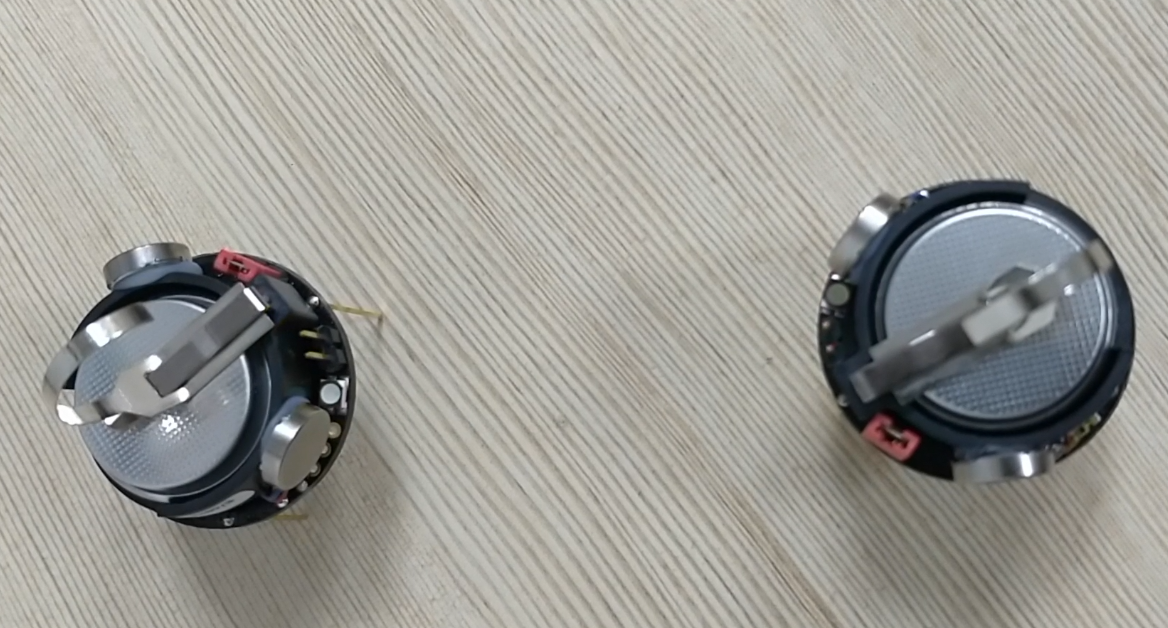
\includegraphics[scale=0.25]{images/communication}}
	\caption{\href{https://photos.app.goo.gl/h2jCY1WrUYU9xLqG8}{Communication between two kilobots [video link]}}
	\label{fig:communication}
\end{figure}

\section{Orbiting of Kilobot}
\subsection{Demonstration}
Video of working demo of problem statement can be accessed using link in figure \ref{fig:orbit}.
\begin{figure}[H]
	\centering
	\fbox{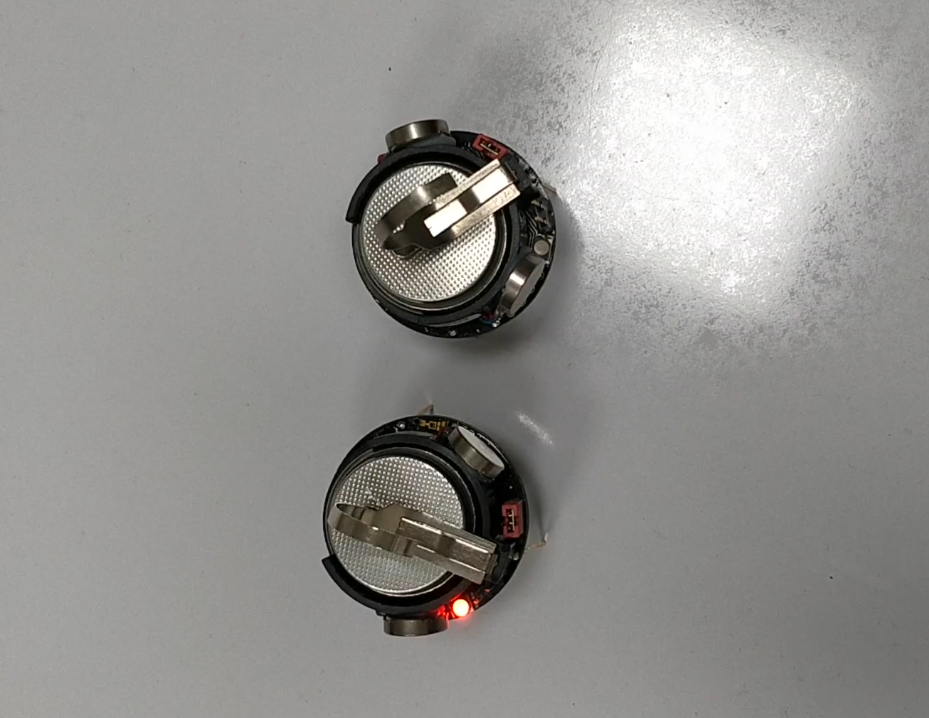
\includegraphics[scale=0.3]{images/orbit}}
	\caption{\href{https://photos.app.goo.gl/xPYoywncwhCk585X8}{Orbiting of kilobot [video link]}}
	\label{fig:orbit}
\end{figure}

\section{Programming Kilobots to move towards the direction of light source}
In this part, our objective is to design an algorithm so that kilobot approaches a source of light (generated by torch light of smartphone) which may be dynamically moving with very slow speed.\\
The problem statement is similar to that of a line follower with just one onboard sensor \cite{simple-line-follower}. The algorithm for single sensor line follower goes as follows:
\begin{enumerate}
	\item Check sensor position.
	\item If sensor is on line, go to step 3 else step 4.
	\item Move right. Go to step 5.
	\item Move left.
	\item Go to step 1
\end{enumerate}
On similar lines, following a light source algorithm is implemented using flowhcart illustrated in Figure \ref{fig:move_towards_light_algorithm}.
\begin{figure}[H]
	\centering
	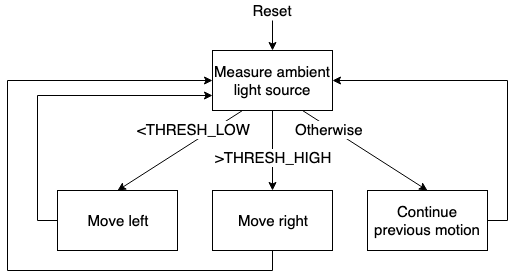
\includegraphics[scale=0.5]{images/move_towards_light_algorithm}
	\caption{Flowchart for move towards light algorithm}
	\label{fig:move_towards_light_algorithm}
\end{figure}
Abovementioned algorithm will help us understand why the robot approaches the source of light in a zig zag fashion. We cannot do significant improvement in algorithm given the limitation of onboard ambient light sensor to one.
\subsection{Demonstration}
Video of working demo of problem statement can be accessed using link in Figure \ref{fig:move_towards_the_light}.
\begin{figure}[H]
	\centering
	\fbox{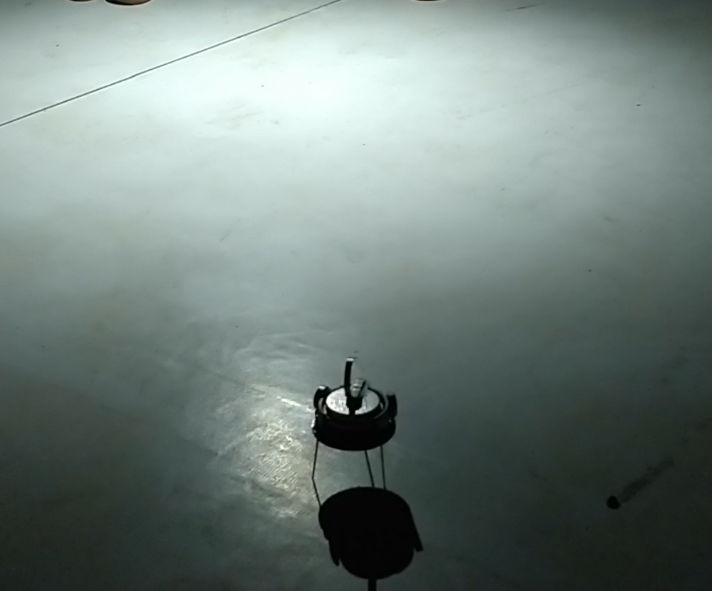
\includegraphics[scale=0.4]{images/move_towards_light}}
	\caption{\href{https://www.google.com/url?sa=j&url=https\%3A\%2F\%2Fphotos.app.goo.gl\%2FnUNghDg4nJygpzUu5&uct=1551610784&usg=G0tZGJ7iMN79F5qGk1QMw5rfodM.}{Move towards the light source [Video link]}}
	\label{fig:move_towards_the_light}
\end{figure}
Different $THRESH\_LOW$ and $THRESH\_HI$ parameters were chosen to implement hysteresis behaviour, thereby, precludingjittery motion.


\section{Synchronizing phase of blinking LEDs}
\textbf{Objective}: Create a logical synchronous clock between different 
robots to allow two or more Kilobots to blink an LED in unison roughly every 4 seconds \\

\noindent A large group of decentralized closely cooperating entities, commonly called a collective or \textbf{swarm}, can work together to complete a task that is beyond the capabilities of any of its individuals \cite{rubenstein2014kilobot}. Following are the three basic swarm behaviors that Kilobots have mastered: 
\begin{enumerate}
	\item  Foraging
	\item  Formation control, and 
	\item Synchronization
\end{enumerate}
Hence, synchronization is one of the swarm behaviours which can be performed by Kilobots. It is often used when coordinating simultaneous
actions between many entities, such as robots or sensor networks.\\

\begin{figure}
    \centering
	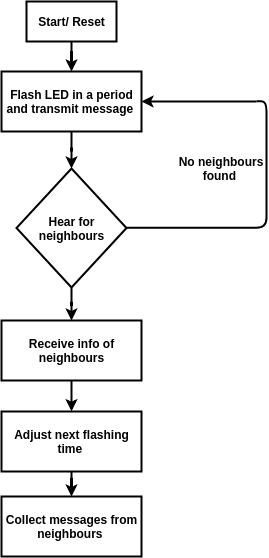
\includegraphics[scale=0.6]{images/sync-algo}
	\caption{Algorithm for synchronizing phase of blinking LEDs }
	\label{fig:sync}
\end{figure}

\noindent For our objective, we will use a method that relies on averaging. The algorithm for Synchronizing robots is given in the flowchart (Figure \ref{fig:sync}).  Each Kilobot acts as an oscillator, flashing its LED in a fixed period \texttt{P}.  At the same time, it continually transmits a message with its current position in the clock period (i.e. a value between \texttt{0} and \texttt{P}.  In the absence of any neighbors, the Kilobot will simply blink in a fixed period, like a firefly.  If the Kilobot hears neighboring Kilobots, then it receives information about their current positions in their own periods. In order to synchronize, it collects that information and uses the average to make an adjustment to its own next flashing time. The steps can be summarized as given below: \\ 

\noindent \textbf{Step 1}: Create a robot oscillator that flashes every 2 seconds.
\begin{verbatim}
#define PERIOD 64
uint32_t reset_time = 0;

// In Program Loop

if (kilo_ticks >= (last_reset + PERIOD)) {
   set LED to red
   last_reset = kilo_ticks
} else {
   turn LED off
}
\end{verbatim}

\noindent \textbf{Step  2}: Let the Kilobot continually transmit the current position of its clock within its ticking period (i.e. \texttt{kilo\_ticks - last\_reset}). Since we reset our clock every 64 ticks, this value will be less than 64. We want this value to be as accurate as possible, so we can read the clock in the \texttt{message\_tx} function. 
\begin{verbatim}
message_t message;

message_t *message_tx() {
    message.data[0] = kilo_ticks - last_reset; // current position in PERIOD
    message.crc = message_crc(&message);
    return &message;
}
\end{verbatim}

\noindent \textbf{Step 3}: Let the Kilobot collect the messages it hears from other neighbors. 
By comparing the its own current clock position to that of its neighbors (i.e. the first byte of the received message), a Kilobot can tell how much it is out of sync with its neighbors. Each time a new message arrives, the Kilobot will store the value of the adjustment to be made. Then, when the Kilobot completes its own time period and flashes, it will also make one big adjustment for next time's flash.

\begin{verbatim}
void message_rx(message_t *m, distance_measurement_t *d)
{
    int my_timer = kilo_ticks - last_reset;
    int rx_timer = m->data[0];
    int timer_discrepancy = my_timer - rx_timer;
    
    // reset time adjustment.
    reset_time_adjustment = reset_time_adjustment + 	rx_reset_time_adjustment;
}
\end{verbatim}

\subsection{Demonstration}
Video of working demo of problem statement can be accessed using link in Figure \ref{fig:sync_lights}.
\begin{figure}[H]
	\centering
	\fbox{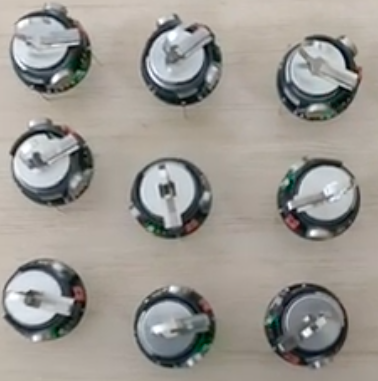
\includegraphics[scale=0.6]{images/sync_lights}}
	\caption{\href{https://photos.app.goo.gl/nvWXb5ziksYnx73s6}{Synchronizing phase of blinking LEDs}}
	\label{fig:sync_lights}
\end{figure}

\bibliography{anurag}{}
\bibliographystyle{ieeetr}
\end{document}
